\section{System design}
Our scatterometer (detailed in Figures \ref{fig:cad} and \ref{fig:light_path}) consists of two mutually coherent, collimated beams of wavelength 532 nm separated vertically by a small angle of approximately $4^\circ$ (assumed to be within the memory effect range for materials of interest). Both beams are attached to a stage that rotates the beams azimuthally about a scattering sample located on the stage's rotation axis. The intensity of scattered light is measured by a stationary camera as the beams are swept through a range of approximately $180^\circ$. The correlation of both beams' speckle images at a given azimuthal angle is proportional to the scattering phase function as a function of angle.

There are three primary components for acquisition. The first is the acquisition camera which we use to record speckle images. The second is the illuminator assembly which adjusts the angular illuminator separation and the azimuthal illumination direction relative to the acquisition camera. The third is the sample assembly which orients and positions the sample such that it is located on the azimuthal rotation axis of the illuminator assembly and maximal light is scattered towards the acquisition camera.
\begin{figure}
    \centering
    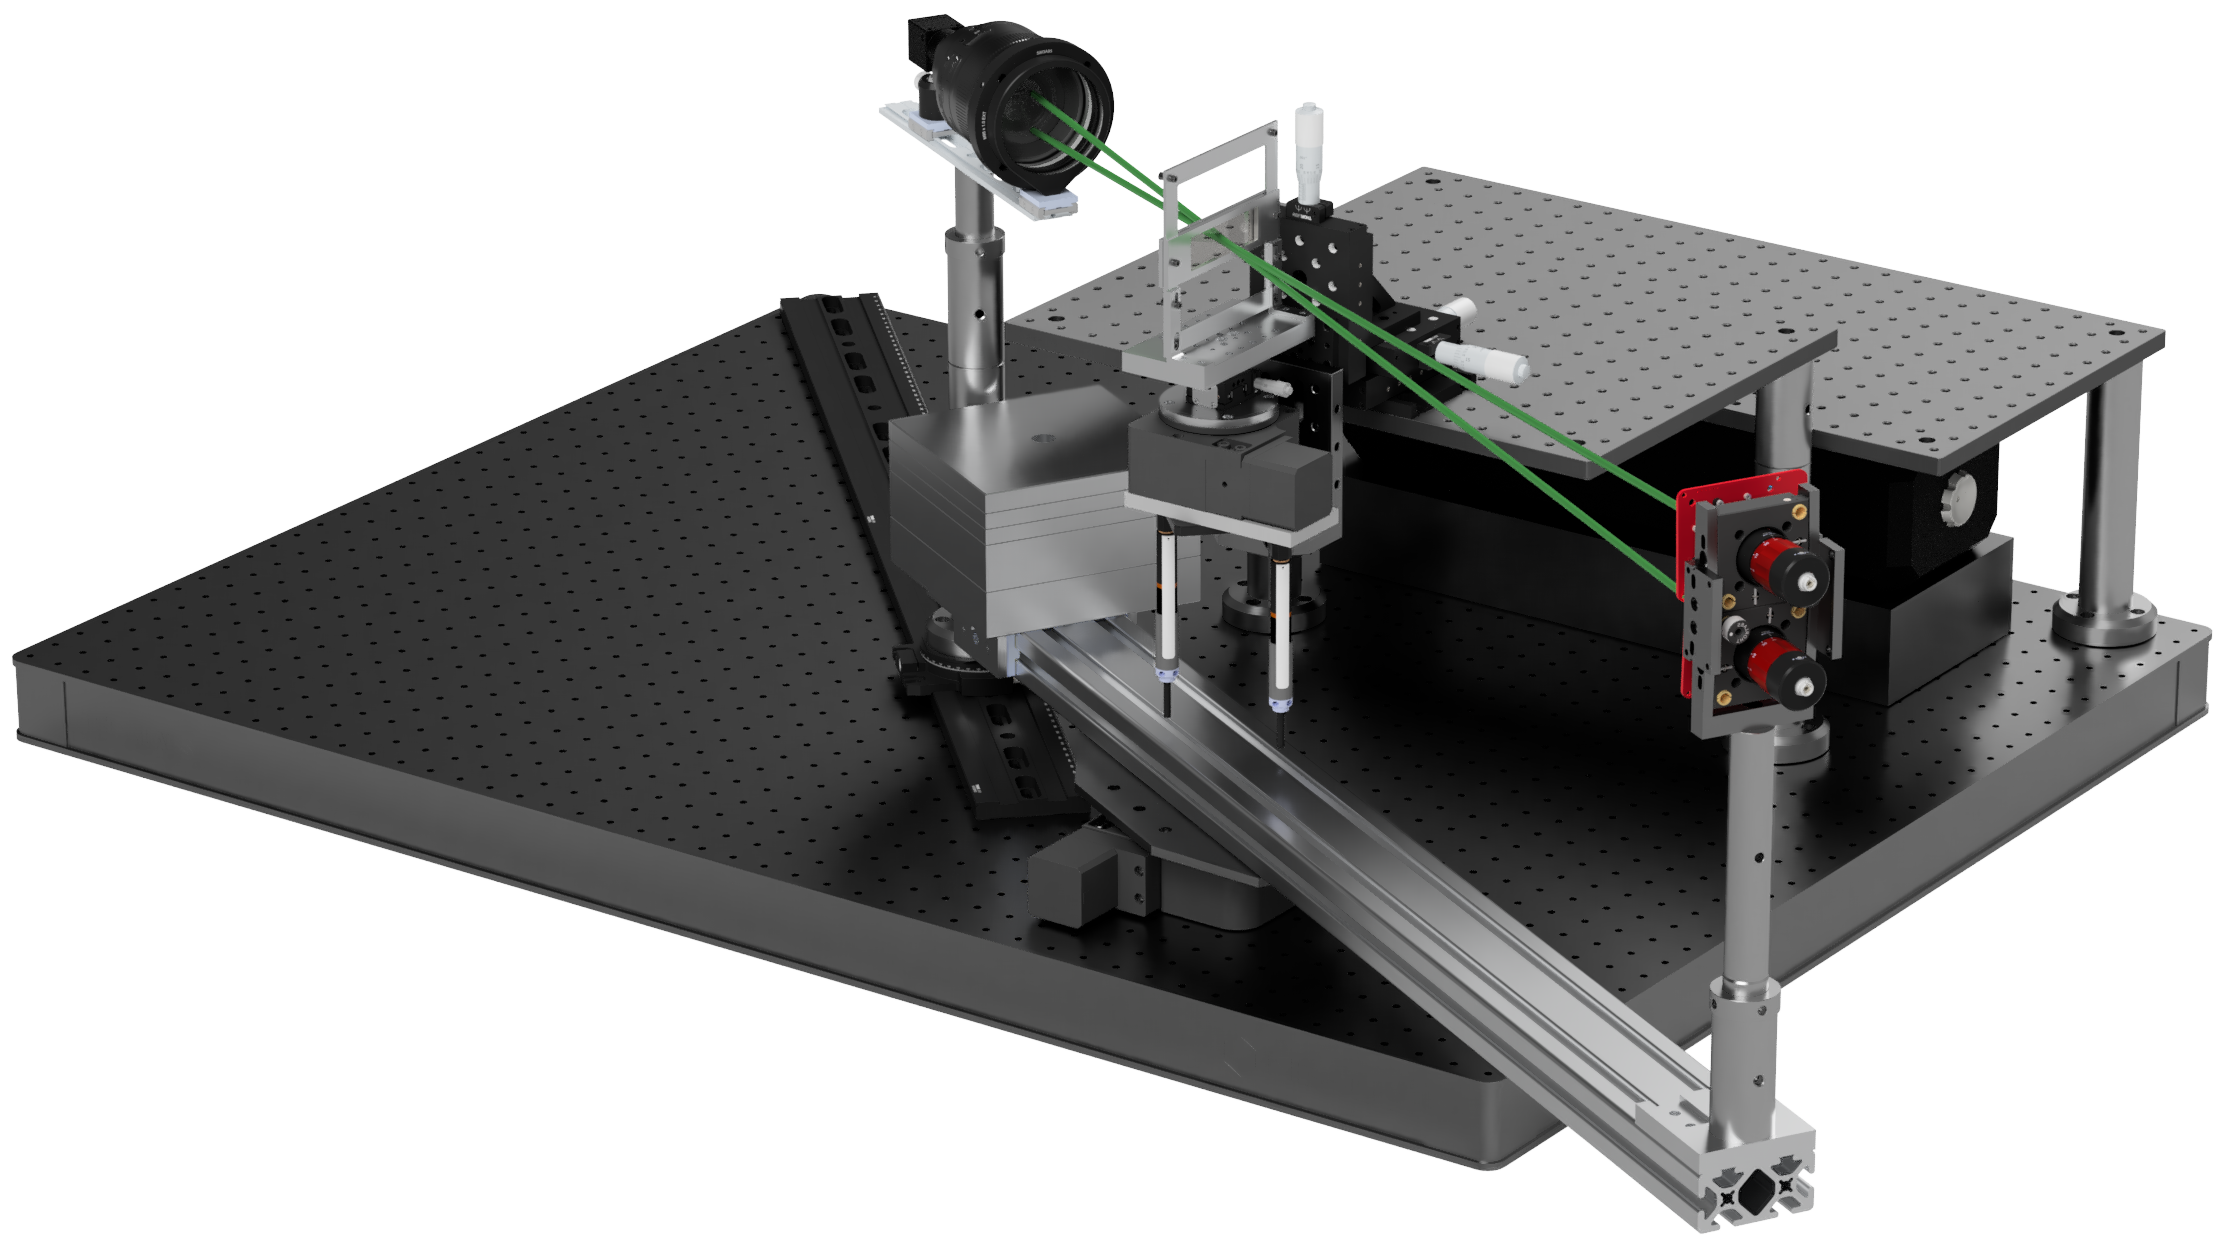
\includegraphics[width=0.75\textwidth]{../figures/setup.png}
    \caption{CAD rendering of speckle correlation scatterometer}
    \label{fig:cad}
\end{figure}

\begin{figure}
    \centering
    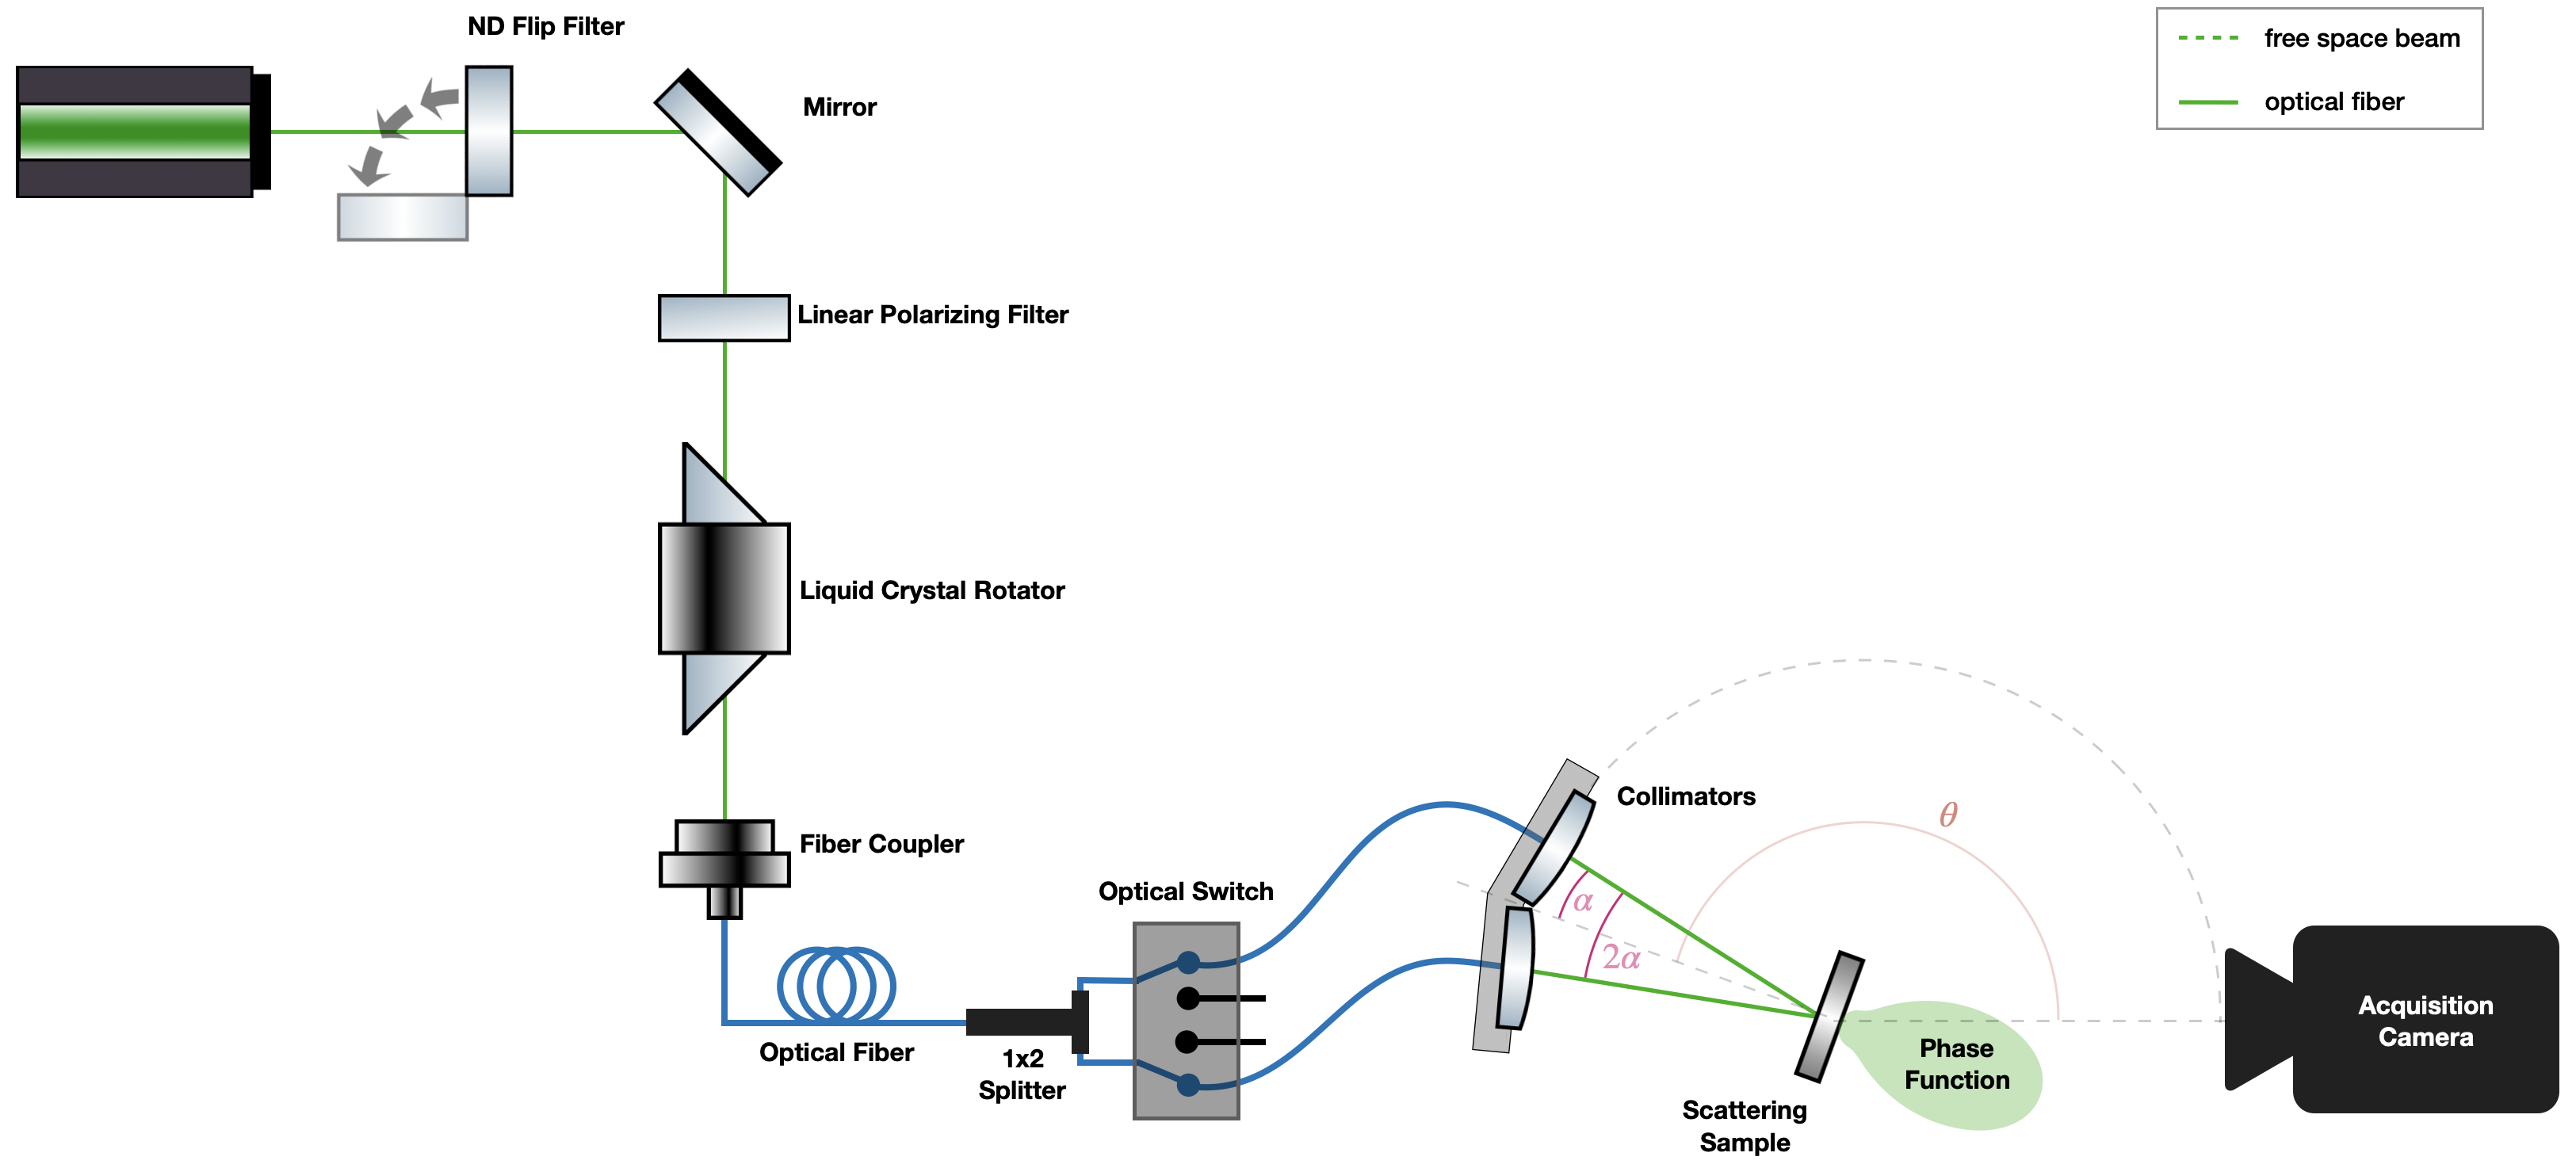
\includegraphics[width=0.75\textwidth]{../figures/laser_path.png}
    \caption{Light path diagram for speckle correlation scatterometer}
    \label{fig:light_path}
\end{figure}

\subsection{Acquisition camera}
The acquisition camera must record high-contrast speckle images and assign directions to light arriving at the camera. A desirable camera and lens combination is one that maximizes angular resolution and light efficiency. Therefore, we choose a camera with a large sensor and small pixel pitch, and a fast lens focused at infinity with a long focal length.

\paragraph{Lens Focal Length} Computing the speckle correlation from images produced by the two illuminators requires both beams to fall within the camera's FOV. Since we maximize single-scattered light by minimizing the illuminator separation, a lens with a small FOV corresponds to illuminators with a small angular separation. However, due to the finite size of the kinematic mounts, there is a minimum vertical separation. This minimum vertical separation and the FOV-limited angle between the beams define a triangle whose length is the distance from the illuminators' kinematic mounts to the scattering sample. An 85 mm lens allows a small beam angle $2.47^\circ$ relative to horizontal and an overall setup size that complies with space constraints.

We use a FLIR Grasshopper scientific camera model GS3-PGE-91S6M-C with an AF-S Nikkor 85mm f/1.4G lens for acquisition.

\begin{table}[htbp]
    \renewcommand{\arraystretch}{1.25}
    \caption{Acquisition camera specifications}
    \begin{center}
        \begin{tabular}{ l l l l l }
        \toprule[2pt]
         \textbf{Property} & \textbf{Spec} \\
         \midrule[0.75pt]
         Camera Model & GS3-PGE-91S6M-C \\
         Resolution & $3376 \times 2704$ \\
         Megapixels & 9.1 \\
         Pitch & 3.69 \si{\micro m} \\
         Sensor & Sony ICX814 \\
         Sensor Type & CCD \\
         Sensor Size & $12 \times 10$ mm \\
         Spectrum & Mono \\
         Lens Make & Nikkor \\
         Lens Focal Length & 85 \si{mm} \\
         Lens Aperture & f/1.4 \\
         Lens Working Distance & $\infty$ \\
         \bottomrule[2pt]
        \end{tabular}
        \label{tab:cpu-gpu}
    \end{center}
\end{table}

\paragraph{Lens Focal Length} Computing the speckle correlation from images produced by the two illuminators requires both beams to fall within the camera's FOV. Since we maximize single-scattered light by minimizing the illuminator separation, a lens with a small FOV corresponds to illuminators with a small angular separation. However, due to the finite size of the kinematic mounts, there is a minimum vertical separation. This minimum vertical separation and the FOV-limited angle between the beams define a triangle whose length is the distance from the illuminators' kinematic mounts to the scattering sample. An 85 mm lens allows a small beam angle $2.47^\circ$ relative to horizontal and an overall setup size that complies with space constraints.

\subsection{Acquisition camera modifications}
The acquisition camera's CCD is protected from debris by a glass window. It is common practice to remove this window under coherent illumination since interference fringes are created when a portion of light passing through the window is reflected internally. However, refraction caused by this window increases the effective focal length of the lens. Camera manufacturers account for this by offsetting the sensor's position along the optical axis so standard lens mounts can be used. Removing the window moves the focus closer to the front of the lens which is an issue when focusing at infinity since the focus will be always located in front of the sensor. The Fotodiox Nik-C (F to C) lens mount consists of a cylindrical component that interlocks with the F lens, and a conical component that matches the camera's C mount threads. To focus at infinity, we shortened the Fotodiox mount by machining 0.5 mm from its conical component to account for removing the glass window. The two lens mount components are secured using four radial screws which must be tightened evenly so their axes are aligned. We designed and 3D printed an alignment fixture that enforces their axial alignment during assembly. See Figure \ref{fig:fotodiox_custom}

\begin{figure}
    \centering
    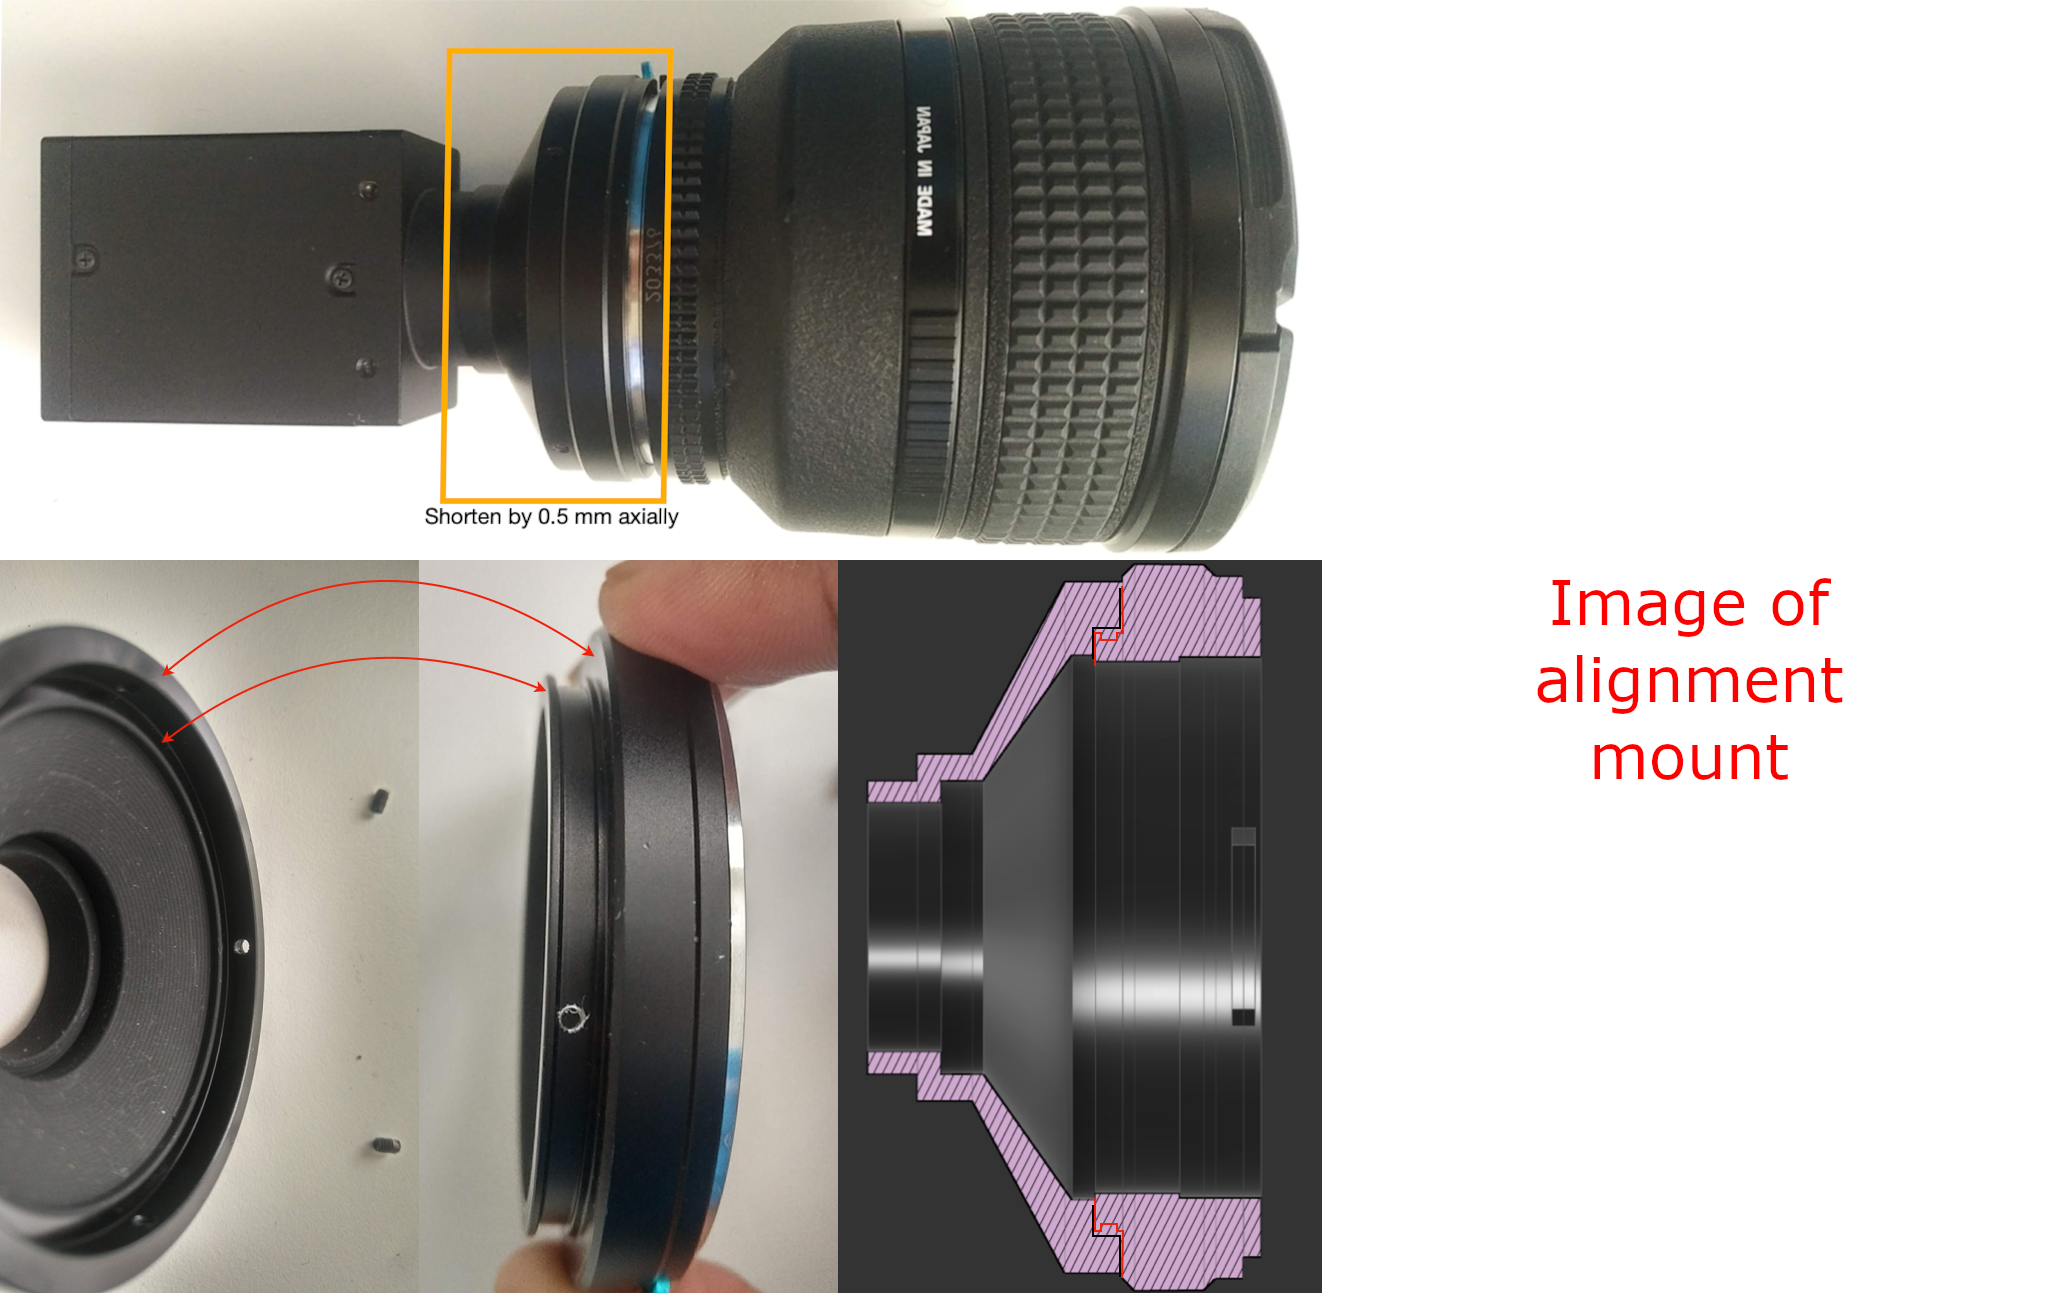
\includegraphics[width=\linewidth]{../figures/F-to-C_mount2.png}
    \caption{}
    \label{fig:fotodiox_custom}
\end{figure}

\subsection{Camera mount}
Mounting the camera to the optical table using the FLIR plastic adapter was not stiff enough and caused the camera to pitch downward over the course of several hours. This was an issue for camera calibration due to pose drift, so we chose to mount the camera via the lens' threads used for attachments.

\subsection{Illuminator Motion assembly}
The illuminator motion assembly controls the illumination beams' directions both in azimuth and elevation. The primary design considerations are high angular resolution and repeatability for fine control of the illumination configuration, and structural stability to minimize vibrations. Each illuminator is attached to a 2-axis kinematic mount that allows $\pm 5^\circ$ in tip and  $\pm 3^\circ$ in tilt. Both kinematic mounts are attached to a custom collimator mount that orients them as close a possible while complying with the FOV constraint of $4.93^\circ$ between the illuminators. The collimator mount is attached to the azimuthal rotation stage via a rail whose length is 2.24 ft (682.85mm). We chose a Thorlabs aluminum extrusion rail since they are designed for modularity. However, the illumination beams experienced large, approximately 2 Hz oscillations when the azimuth stage moved. Modular aluminum extrusions have cross-sections that make them light-weight but at the cost of having low bending and torsional stiffness. This means they behave as springs when cantilevered with large weights are attached at the end. The angular displacement of a beam with length L due to an external torque T is
%
\begin{equation}
    \tau = \frac{TL}{GI}
\end{equation}
%
where G is the elastic modulus which is determined by the material of the beam, and I is the torsional moment of inertia determined by the beam's cross-section profile. The beam length is fixed due to setup geometry, as well as the elastic modulus since the extrusion is made of aluminum. The external torque is generated when the azimuth stage accelerates due to the collimator mount's inertia, so we want to choose the cross-section profile that maximizes the torsional moment of inertia. Torsional moment of inertia increases proportionally to the length of the longest connected path in a cross-section profile, but it can only be calculated analytically for a narrow class of profiles. We performed finite element analysis (FEA) to assess a variety of Thorlabs and 80/20 extrusions. The results in Figure \ref{fig:beam_torsion} show that 80/20 extrusions outperformed Thorlabs extrusions, and a small aspect ratio reduces beam deflection by two orders of magnitude. We chose the 80/20 1530-S extrusion. This has a 1:2 aspect ratio with sufficient torsional stiffness without violating space constraints.
%
\begin{figure}
    \centering
    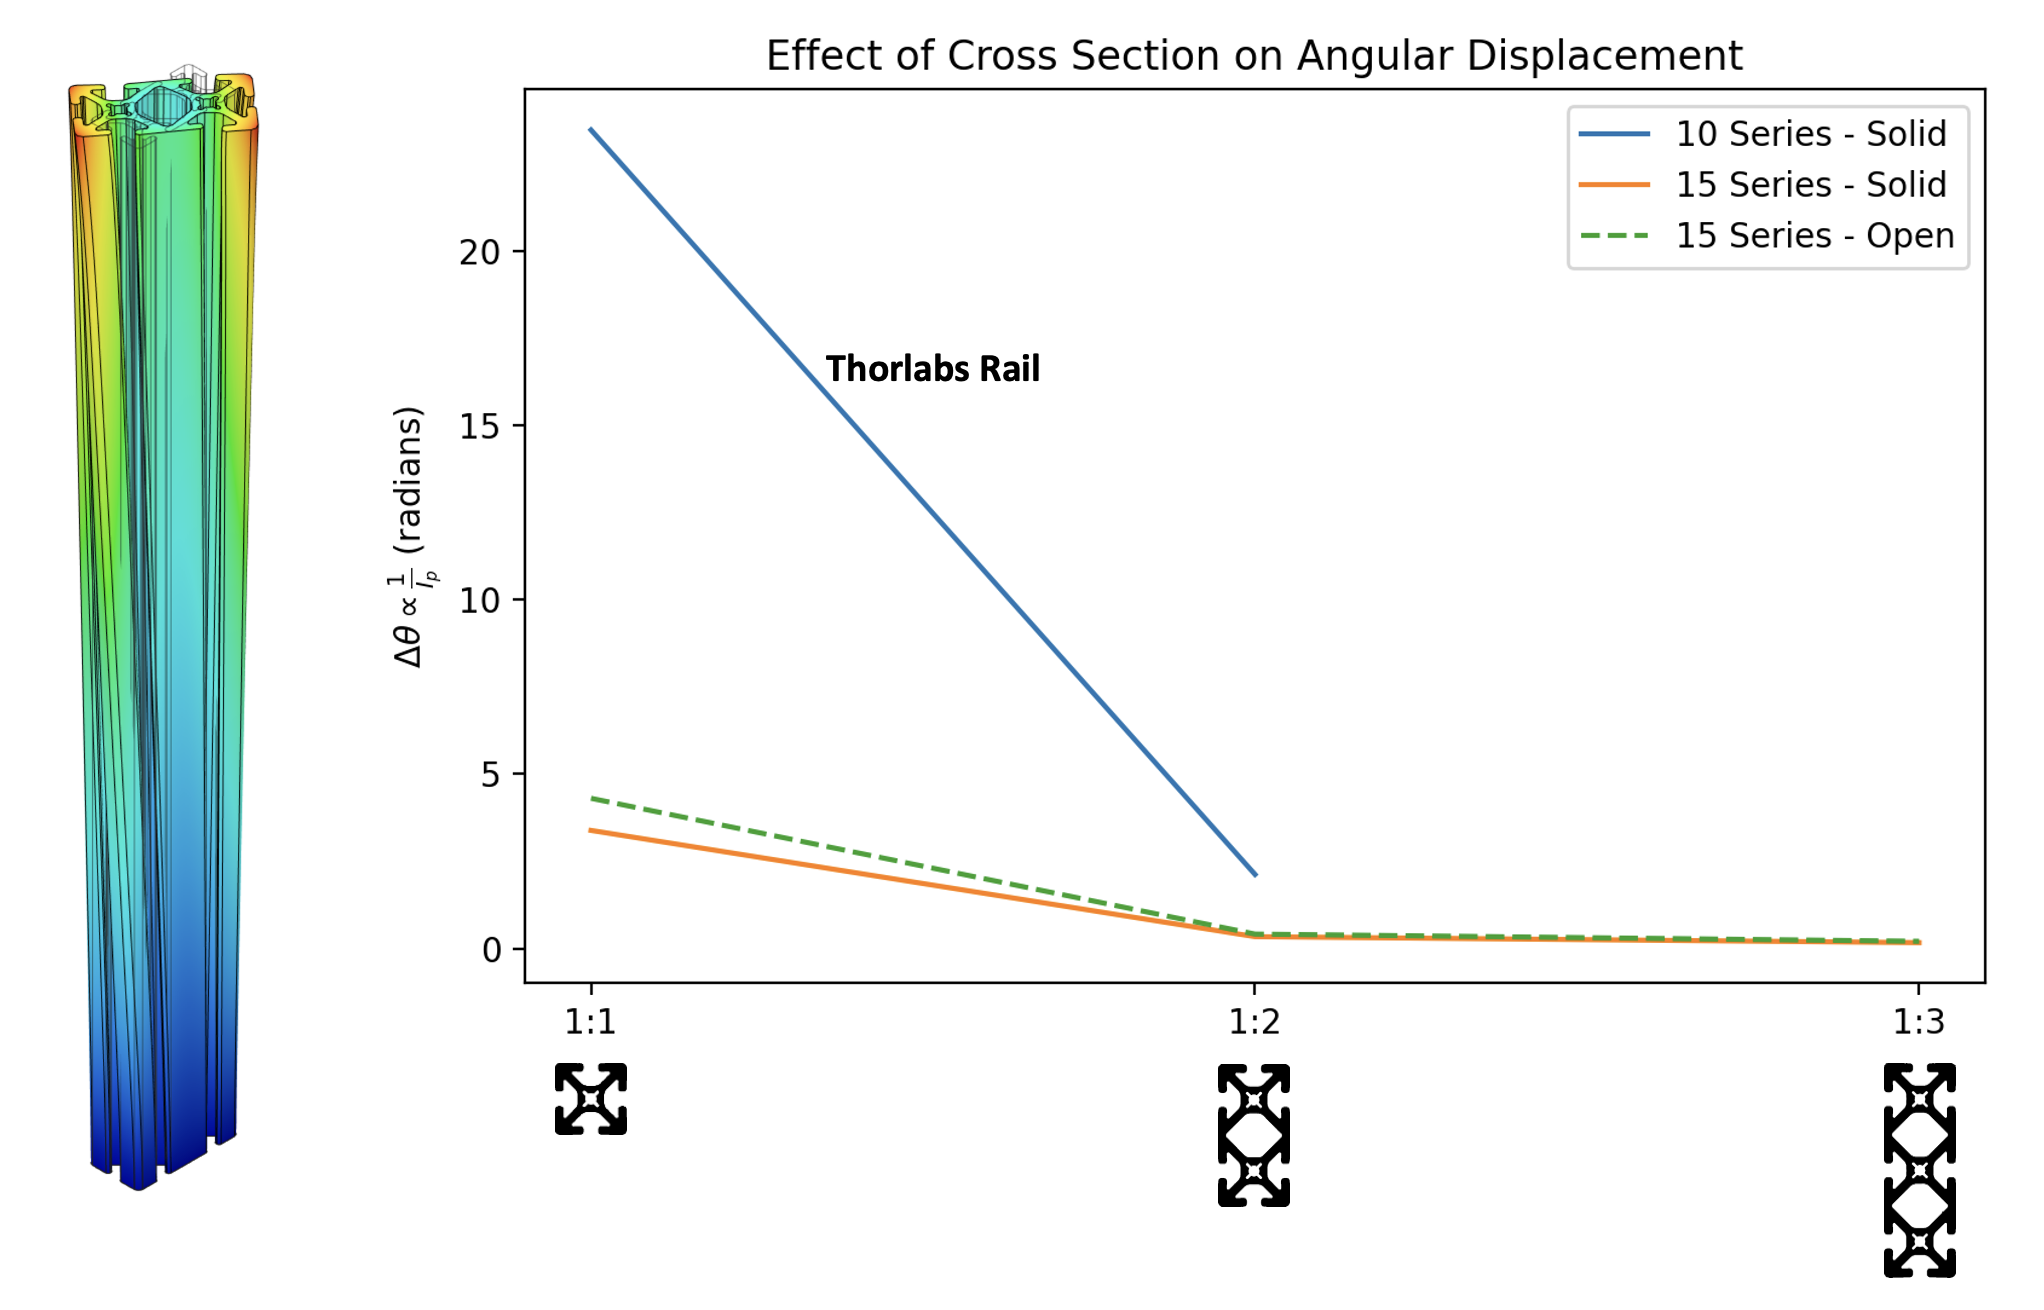
\includegraphics[width=0.75\linewidth]{../figures/beam_torsion.png}
    \caption{Left: FEA beam torsion; Right: FEA beam deflection analyses indicate 80/20 rail perform significantly better than Thorlabs optical rails, and that angular beam deflection decreases for decreasing cross-section aspect ratio.}
    \label{fig:beam_torsion}
\end{figure}


\subsection{Collimator Mount}
Calculates the design space for the collimator mount.
Given acquisition camera position and FOV, it calculates valid combinations of 
    1) linear collimator separation
    2) angular collimator separation
$d_camera = 969.417$ mm
$r_aperture = 26.73$ mm

\begin{figure}
    \centering
    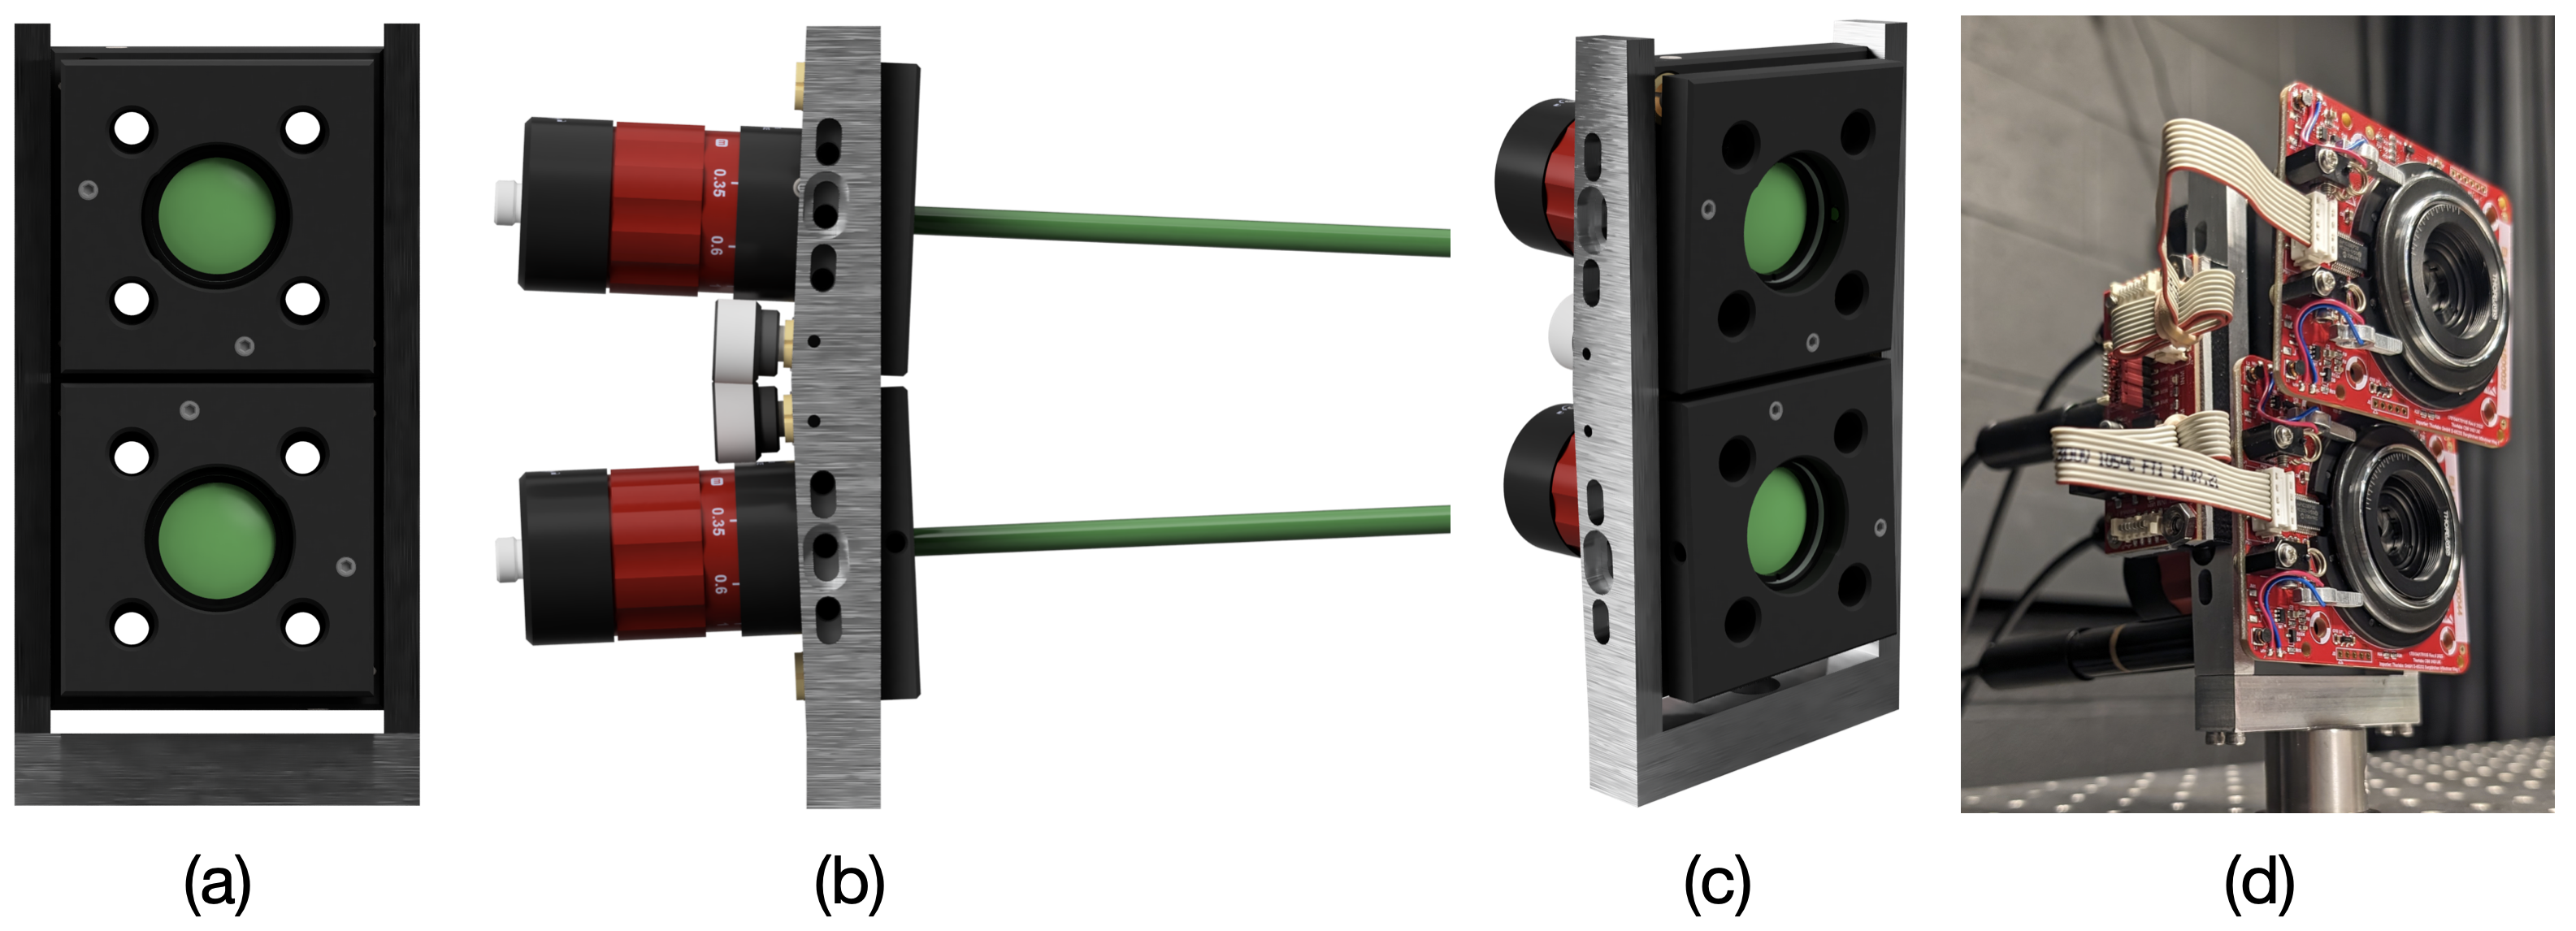
\includegraphics[width=\linewidth]{../figures/collimator_assembly_summary.png}
    \caption{(a) CAD front view of collimator mount; (b) CAD side view showing the relative orientations of illumination beams; (c) CAD perspective view; (d) Fully assembled collimator mount which controls vertical and angular illuminator separation. Beam diameter is also controlled using motorized iris diaphragms.}
    \label{fig:collimator_mount}
\end{figure}

\subsection{Sample assembly}
The sample motion assembly's primary purpose during acquisition is to rotate the scattering sample so the amount of laser light scattered towards the camera is maximized since there are transmittive losses at air-glass interfaces as the illuminators' azimuthal position changes. This rotation is controlled by a small rotation stage which is mounted on an XYZ stage and an tip/tilt stage. These additional stages are used to control the rotation stage's orientation so it can made to be collinear with the illuminator assembly's azimuthal rotation axis. There is an additional translation stage mounted to the rotation stage's motion plate that is used to align the center of a mounted sample with the upper- and lower motion stages' rotation axes.
\begin{figure}
    \centering
    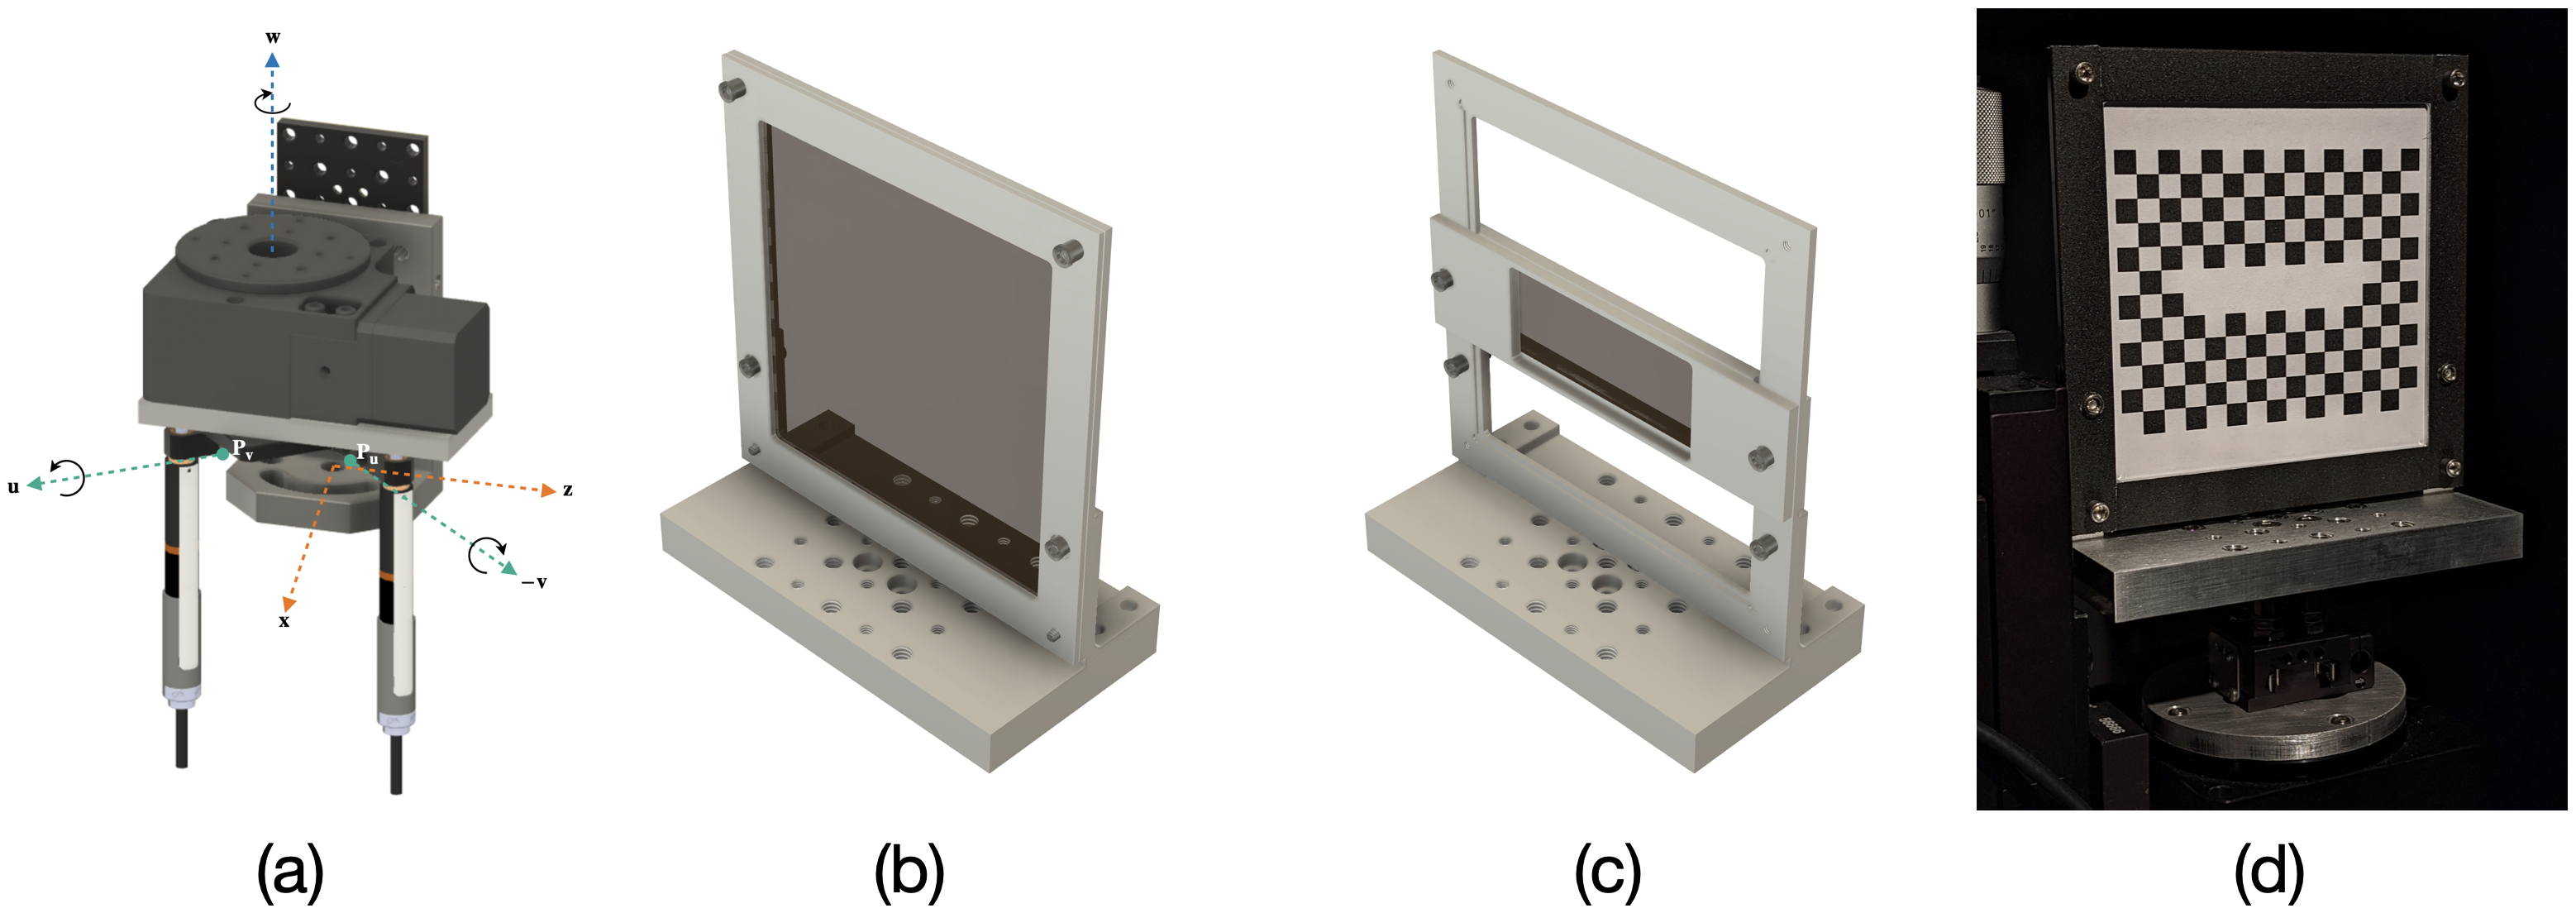
\includegraphics[width=\linewidth]{../figures/sample_assembly_summary.png}
    \caption{(a) Sample motion assembly without sample mount; (b) Sample mount configured for calibration target (not drawn to scale with respect to (a)); (c) Sample mount configured for scattering sample on a microscope slide (not drawn to scale with respect to (a)); (d) Sample mount shown on top of sample assembly with calibration target installed}
    \label{fig:sample_motion_assy}
\end{figure}

The sample mount is a custom, dual purpose mount used to hold scattering samples during acquisition and checkerboard targets during calibration. It is designed such that the front face of a calibration target is in the same plane as the central plane of a scattering sample. It consists of a base and angle mounts used to attach a square aluminum frame that holds a $10 \times 10$ cm glass window in place through compression by tightening four thumbscrews. Scattering samples are mounted by removing the aluminum frame's front face and attaching an inset frame that holds microscope slides via compression.

\section{Sample Analysis Station}
We characterize each scattering sample by measuring its optical density and its particle density along its thickness. We measure optical density by comparing the power of ballistic laser laser before and after it has passed through a scattering sample. The laser is the same wavelength as the acquisition laser, and images are acquired using a Point Grey GS3-PGE-91S6M-C scientific camera with an AF Micro-Nikkor 200mm f/4D focused at infinity. We measure particle density as a function of depth by computing particle area density for each image in a focal stack. The microscope imager is an Allied Vision Prosilica GT3400 scientific camera whose lens consists of a Canon 180mm f/3.5 L EF Macro lens and a 0.65NA 40X Olympus Plan Achromat Obective
\begin{figure}
    \centering
    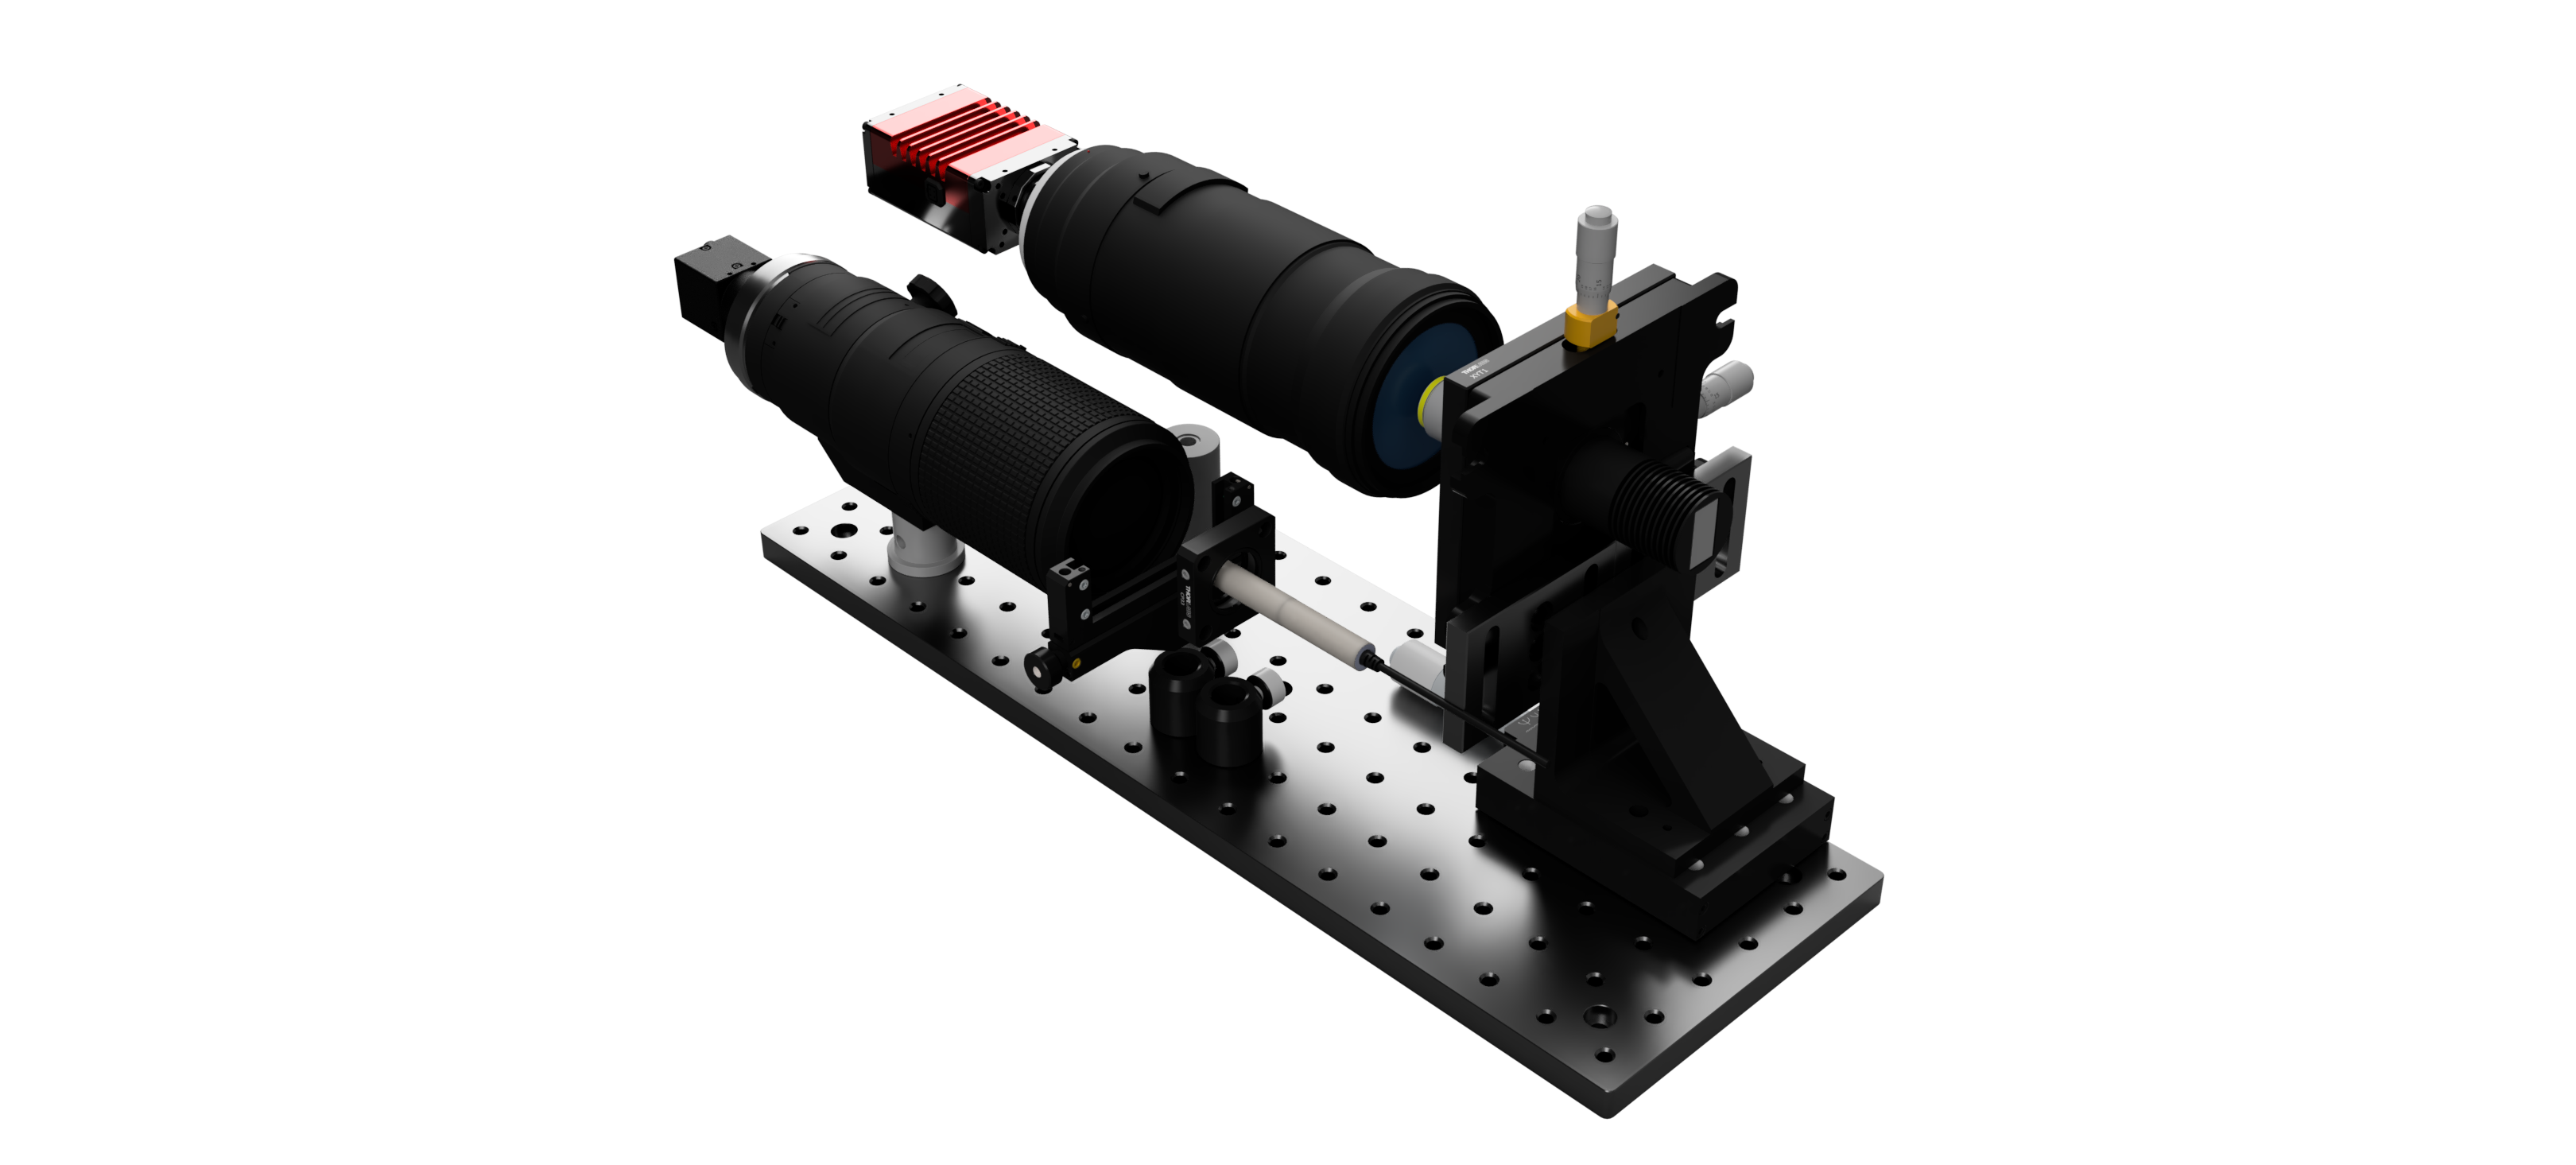
\includegraphics[width=\linewidth]{../figures/SampleAnalysisStation.png}
    \caption{CAD rendering of the sample analysis station}
    \label{fig:sample_analysis_station}
\end{figure}